\section{Localisation and World Modelling}
\label{sec:Localisation}
The localisation for 2009 was based on the Unscented Kalman Filter (UKF) used in 2008 \cite{NUManoids2008}. A number of extensions were made to improve upon the previous years implementation. Changes were made to include newly available information due to advances in vision, as well as to make use of ambiguous data that was previously available but not used.

\begin{table}
\centering
\begin{tabular}{|l|l|l|l|}
\hline
state & units & Description \\ \hline
x & cm & Robot�s own x-coordinate \\ \hline
y & cm & Robot�s own y-coordinate\\ \hline
$\theta$  & radians & Robot�s orientation\\ \hline
xb & cm & Ball x-coordinate\\ \hline
yb & cm & Ball y-coordinate\\ \hline
vxb & cm/sec & Ball x velocity\\ \hline
vyb & cm/sec & Ball y velocity\\ \hline
\end{tabular}
\caption{States estimated by the Unscented Kalman Filter}
\label{states}
\end{table}

\subsection{UKF Updates}
There are a total of four different update types that are performed, depending on the information available and its source. It is important that these updates be done in the correct order so that the information is interperetted correctly. 

Time updates must be done before anything else. This is done so that the robots estimate is fully updated before object updates are done. If this were not the case and for example odometery data was applied after the object updates, the object updates may have adjusted the estimated position correctly and the odometery would then change this estimate decreasing its accuracy.

Shared mobile object updates are performed second. These are currently done only when there is no locally available data on the object. These measurements have no reliance on any of the other information gathered. They do not depend on the position of this robot since they refer to an exact field location.

The Fixed object updates are done next. The fixed objects are used to determine the robots position. While the mobile objects primarily determine the location of the respective object. Their absolute position is determined by using their position realative to the estimated robot position. Therefore in order to have the best estimate for the mobile objects position we should start with the most up to date estimate of the robots position.

Mobile object updates are left until last. As this is only currently used for the ball, it is a much higher priority that the relative position of the ball coming from the world model stay accurate. Therefore the current robot estimate is found and the position field position of the ball is then found from the relative information based on this.

\subsubsection{Time Updates}
Time updates occur every robot frame. They run at a consistant time step and use information that is always available. There are two main time based updates performed. One based on odometery data, the second to update positions based on the estimated velocities.

Firstly the odometery data is used to update the model. This will update the x, y and $\theta$ states based on the motions that the robot has performed. Following this the position coordinates of the ball (xd and xy) are adjusted based estimated velocity (vxb and vxy). The estimated velocity then suffers from decay to account for friction and the time update is completed.

\subsubsection{Fixed Object Updates}
Fixed object updates occur when an object known to be fixed on the field has been recognised. The update will modify the estimated x, y and $\theta$ states.

\subsubsection{Mobile Object Updates}
Mobile object updates are used for objects that are not fixed to the field. Currently used only for the ball. When a mobile object update is done the estimate for the location of that object, that objects velocity, as well as the current x, y and $\theta$ state estimate for the robot are updated.

\subsubsection{Shared Mobile Object Updates}
Shared mobile object updates are preformed when using state estimate information on a mobile object that has been provided by another robots model. The shared object update uses the estimated as well as the variance information. Simliarly to the mobile object update the local estimates of the states are updates, as well as the current x, y and $\theta$ state estimates.

\subsection{Multiple Models}
The current robocup field contains many ambiguous points of reference as can be seen in \autoref{fig:LocalisationPoints}. When multiple ambiguous points are found it is possible to use a simple decision tree to determine which objects these are, however there are often times not enough objects are seen or the decision is still unclear. The World Model was therefore extended to incorporate multiple UKF models to allow for the use of ambiguous measurements. The method used to implement the multiple models is similar to that used with an Extended Kalman Filter (EKF) described in \cite{QuinlanMiddleton09}.

The basic idea is that when an ambiguous object is seen e.g. a yellow goal post, we can determine that there are a number of possible fixed objects that could have been seen, in this example the left yellow post or the right yellow post. Using a multiple models approach the current model is cloned to create as many models as there are options, in our example two models will be created. One model is then updated with the first option the next model with the second and so forth.

As these updates are done an $\alpha$ variable is modified depending on how well the update fits the previous model. The larger the discrepancy the more the $\alpha$ value is reduced. Therefore the model with the largest $\alpha$ value following the update can be deemed to have been updated with the most likely option and therefore be the most correct model. This process can be repeated for multiple ambiguous options and therefore the results of all possible combinations can be found.

If this process were repeated again and again, we would end up with an exponentially growing collection of UKF models filling up memory and taking up processing time. Therefore it is also necessary to merge these models, combining two models into one. Merging is done so that information is not lost.

\begin{figure}[htpb]
\begin{center}
    \scalebox{0.5} {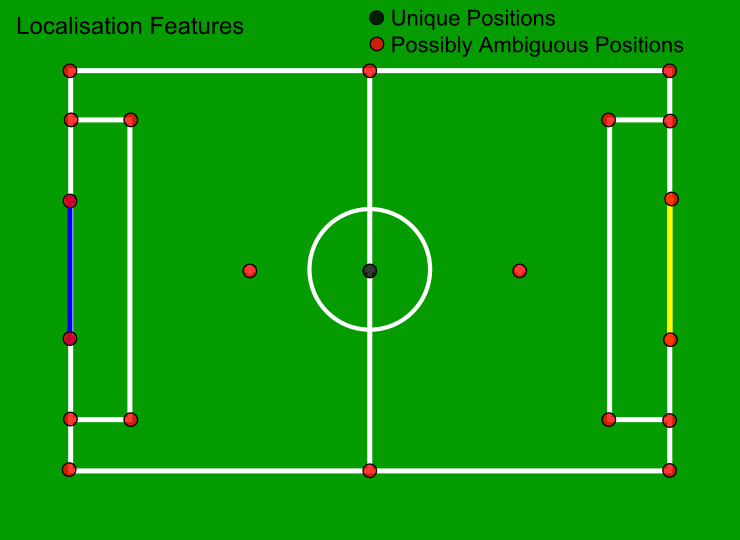
\includegraphics{figs/LocalisationPoints.png} }
    \caption{Available localisation landmarks}
    \label{fig:LocalisationPoints}
\end{center}
\end{figure}

\subsubsection{Intelligent Model Resets}
One advantageous way of using the multiple models structure is to automatically introduce multiple models when uncertainty arises. This has currently been done in two ways. 

Firstly when the world model initially starts and whenever it is reset. Mutiple models are created, spread around the field in likely starting locations as shown in \autoref{fig:PlayerResetModels}. For example a model is created in each goal area pointing towards the center of the field to represent the scenario of a goalkeeper being booted in the goals. By creating all of these likely scenarios, once the robot starts to receive update information the model that best allows for this information is quickly selected. This model then converges much more quickly than if a single highly uncertain model were created at the start.

\begin{figure}[htpb]
\begin{center}
    \scalebox{0.30} {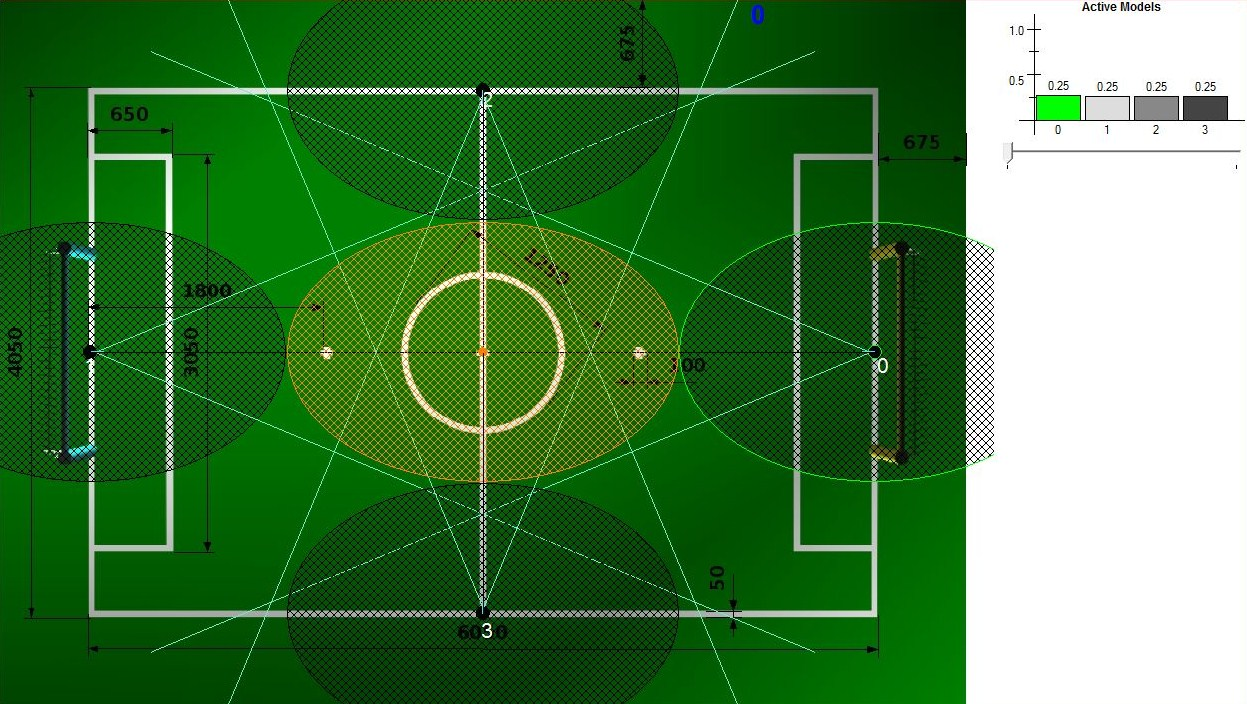
\includegraphics{figs/PlayerResetModels.JPG} }
    \caption{Player Reset Models}
    \label{fig:PlayerResetModels}
\end{center}
\end{figure}

Secondly, penalties inflicted during a game, once completed will send the robot to either of the restart positions situated on each side line at middle of the field. The robots are restarted facing towards the center of the field. Therefore the robots starting state can be narrowed down to two possible options. Two models are therefore created, one for each option as shown in \autoref{fig:PenaltyResetModels}. This allows the robot to find the correct model extremely quickly with only a few glimpses of a goal object required.

\begin{figure}[htpb]
\begin{center}
    \scalebox{0.30} {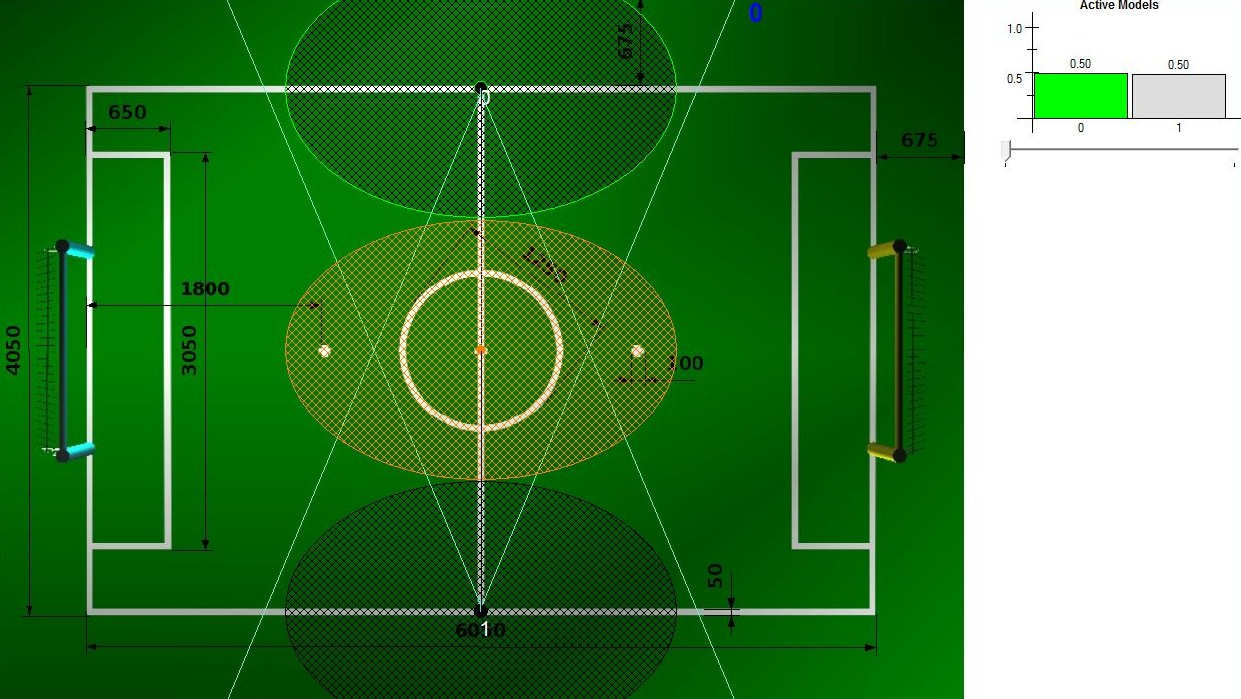
\includegraphics{figs/PenaltyResetModels.JPG} }
    \caption{Penalty Reset Models}
    \label{fig:PenaltyResetModels}
\end{center}
\end{figure}

\subsection{Outlier Detection}
Outliers are updates that have been deemed to be too far removed from the current model given its current state and estimated error region. Outliers are used to reduce the impact of the false positive object recognition case, and are used to detect the kidnapped robot scenario.

When an update is detected as an outlier the update is not performed on the model, this stops the outlier from ruining an otherwise accurate model. An outlier counter for this update type is then incremented to indicate that an outlier has been detected. This counter decays over time and is use to detect the kidnapped robot scenario. Once the combined outlier counter of all update types exceeds a tunable average value of outliers per second threshold, the kidnapped robot scenario is triggered.

Once a kidnapped robot state has been detected a local reset is done on both x,y positional state and the heading state. During the reset the variance of the robots position in terms of each of this state is greatly increase, therefore allowing new incoming updates to greatly modify this current model and not be detected as an outlier.

\subsection{Additional Objects}
Some new objects were available as inputs for localisation this year that were not available in previous years. These included the centre circle and the penalty spots. These newly available landmarks saw huge improvements in positioning when in the mid-field area as there was previously a distinct lack of landmarks once you moved away from the goal areas. The middle of the center circle provides one of the few unique landmarks available. While the penalty spots can represent one of two locations and therefore can make use of multiple models if simple hueristics prove fruitless.
